\documentclass{article}

\usepackage[T1]{fontenc}
\usepackage[utf8]{inputenc}
\usepackage[frenchb]{babel}
\usepackage{fullpage}
\usepackage{graphicx}
%\usepackage{layout}
%\usepackage{geometry}
%\usepackage{setspace}
%\usepackage{soul}
%\usepackage{ulem}
%\usepackage{eurosym}
%\usepackage{bookman}
%\usepackage{charter}
%\usepackage{newcent}
%\usepackage{lmodern}
%\usepackage{mathpazo}
%\usepackage{mathptmx}
\usepackage{url}
%\usepackage{verbatim}
%\usepackage{moreverb}
%\usepackage{listings}
%\usepackage{fancyhdr}
%\usepackage{wrapfig}
\usepackage{color}
%\usepackage{colortbl}
\usepackage{amsmath}
\usepackage{amssymb}
\usepackage{amsfonts}
%\usepackage{mathrsfs}
%\usepackage{makeidx}
%\usepackage{parskip}
\usepackage{titlesec}
\usepackage{hyperref}

% pour compiler: 

% faire    pdflatex ex-rapport
% (si les references aux numeros de parties apparaissent comme des
% "?", recompiler une fois)

% la compilation de la bibliographie est davantage une "incantation":
% faire     bibtex ex-biblio
% puis      pdflatex ex-rapport (un nombre premier de fois)


\title{ \Huge{Rapport Projet 2} \\ Où l'on parle de rongeurs}
\author{Guillaume Coiffier - Léo Valque}
\date{2017}

\titleformat{\part}[display]
  {\normalfont \huge \bfseries \centering}
  {\partname \thepart}{20pt}{\Huge}

\newcommand{\non}[1]{\overline{#1}}

\begin{document}

\renewcommand{\labelitemi}{$\bullet$}

\maketitle
\tableofcontents
\newpage

\part{Généralités}

\section*{Remarques générales}

\begin{itemize}
 \setlength\itemsep{3pt}
 \item \textbf{Niveau du binôme :} Intermédiaire
 \item \textbf{Adresse du dépôt Git :} \url{https://github.com/GCoiffier/Projet-2}
 \item Les fichiers de tests sont situés dans le dossier Programs. Les fichiers contenant du code fouine ont une extension \texttt{.ml}
 \item Les fichiers compilés pour la machine SECD sont situés dans le dossier Stack\_Programs. Ils ont une extension \texttt{.code}
 \end{itemize}

\section{Comment exécuter notre programme}

\subsection{Avec Linux}

\begin{itemize}
  \setlength\itemsep{3pt}
 \item Pour compiler le programme, utilisez simplement la commande \texttt{make}. Celle-ci crée un exécutable appelé \textit{fouine}.
 \item Pour nettoyer le répertoire de travail, utilisez la commande `make clean`.
 \item \texttt{./fouine fichier} exécute le code contenu dans **fichier** et renvoie le résultat de ce code (qui doit être un entier)
 \item \texttt{./fouine -debug fichier} commence par afficher le code parsé dans la console, puis exécute le code et affiche le résultat.
 \item \texttt{./fouine -interm sortie fichier} compile le code parsé et le stocke dans sortie. Si aucun fichier de sortie n'est spécifié, le programme affichera le code dans la console.
 \item \texttt{./fouine -machine fichier} compile le code parsé et effectue l'interprétation mixte : ce qui peut être exécuté sur la machine à pile y est exécuté, le reste fait appel à l'interpréteur standard. Le code en entrée doit être un code fouine.
 \item \texttt{./fouine -execute fichier} compile le code parsé et l'exécute sur la machine à pile. Ce code doit être dans le langage de la machine à pile.
 \item \textbf{NB :} il est dans tous les cas possibles de ne pas donner de fichier d'entrée à fouine. Le programme s'éxecute alors en mode interactif et il faut entrer un programme dans la console.
\end{itemize}

\paragraph{Exemples :}

\texttt{
\begin{itemize}
 \setlength\itemsep{3pt}
 \item[>] ./fouine
 \item[>] ./fouine Programs/factorielle.ml
 \item[>] ./fouine -debug Programs/function.ml
 \item[>] ./fouine -interm
 \item[>] ./fouine -interm toto.code Programs/prog1.ml
 \item[>] ./fouine -execute toto.code
 \item[>] ./fouine -machine Programs/prog2.ml
 \item[>] ./fouine -debug Programs/function.ml
\end{itemize}
}

\subsection{Avec un autre OS}

\begin{enumerate}
 \item Installez Linux
 \item Reprendre les instructions de la section précédente.
\end{enumerate}


\section{Fouine}

\subsection{Fouine}
La fouine (Martes foina) est une espèce de mammifères carnivores d'Europe et d'Asie, au pelage gris-brun, courte sur patte et de mœurs nocturnes. C'est une martre (ou marte) faisant partie de la famille des Mustélidés, au même titre que la belette, le blaireau, la loutre, le putois ou le furet, petits mammifères carnivores se caractérisant souvent par leur odeur forte.

\begin{figure}[ht]
\centering
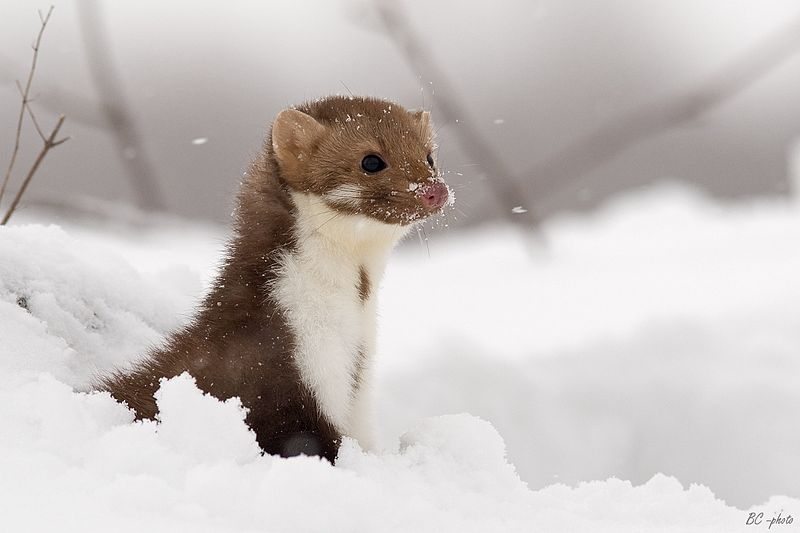
\includegraphics[width=8cm]{fouine_hiver.jpg}
\caption{Fouine photographiée en hiver en République tchèque.}
\end{figure}

Les fouines sont des animaux solitaires, comme la plupart des autres espèces de martres. Elles évitent leurs congénères en dehors des périodes de reproduction. Il s'agit d'animaux territoriaux qui marquent leur territoire avec des secrétions et le défendent au moins contre d'autres fouines de même sexe. La grandeur du territoire est variable, mais reste inférieure à celui de la Martre des pins. Leur grandeur va de 12 à 21cm et varie en fonction du sexe (les territoires des mâles sont plus grands que ceux des femelles), de la saison (ils sont plus petits en hiver), de l'habitat (ils sont plus grands en campagne qu'en ville) et de la nourriture disponible. Leur activité est surtout nocturne. L’espérance de vie de la fouine est d’approximativement douze ans. \\ ~ \\

\textit{Extraits de l'article de Wikipedia \cite{WikiFouine}}

\subsection{Le langage Fouine}

Le langage fouine est un langage de programmation constituant un sous-ensemble du langage Ocaml. Il comprend notamment :
\begin{itemize}
 \item Les expressions arithmétiques et booléennes
 \item Les déclarations de variables et de fonction (syntaxe \texttt{let ... = ... in ...})
 \item Les branchements conditionnels
 \item Les fonctions récursives (syntaxe \texttt{let rec ... = ... in ...})
\end{itemize}

Mais, à la différence d'Ocaml, il ne comprend pas :
\begin{itemize}
 \item De typage : toutes les fonctions prennent en argument des entiers, et renvoient des entiers
 \item De structures de données telles que les listes
 \item De filtrage par motif
 \item La couche orientée objet
\end{itemize}

Cependant, nous verrons que fouine peut être étendu avec certaines fonctionnalités, notamment un système de gestion d'exceptions et des références.\\
Ce langage ne figure cependant pas dans la liste des 700 langages de programmation proposée par Peter J. Landin \cite{700}.

\section{Organisation du rapport et du projet}

\subsection{Organisation du rapport}

Ce rapport s'organise en 3 parties, si l'on exclut cette partie d'introduction. \\
Dans un premier temps, nous parlerons de l'interpréteur fouine, de ses fonctionnalités et de certains aspects importants de son implémentation. \\
Dans un second temps, nous parlerons de la machine à pile SECD, également implémentée par nos soins. \\
Enfin, la dernière partie sera consacrée à l'exécution mixte fouine/SECD d'un code.

\subsection{Organisation du projet}



\subsection{Avancement du projet en fonction du temps}
\subsubsection*{Rendu 2}
\begin{itemize}
 \item \textbf{Semaine 1} 
    \begin{itemize}
    \item Lexer et parser de base

    \item Définition d'un type programme pour les programmes fouine

    \item Interprétation des fichiers fouine sans les fonctions
      (ie expressions arithmétiques, booléennes, \texttt{if ... then ... else} et \texttt{let ... in})
    \end{itemize}
    
  \item \textbf{Semaine 2 }
    \begin{itemize}
      \item Interprétation des fichiers fouine avec des fonctions
      \item Interprétation des fichiers fouine avec des fonctions récursives
    \end{itemize}
  
  \item \textbf{ Semaine 3 }
    \begin{itemize}
    \item Gestion des exceptions
    \item Gestion des références
    \item Gestion du \texttt{begin...end} et du \texttt{let \_ = ...}
    \item Ajout de primitives "bonus" \texttt{prStr} (qui renvoie 0 et affiche une string) et \texttt{prNl} (qui passe une ligne et renvoie aussi 0)
    \end{itemize}
\end{itemize}

\subsubsection*{Rendu 3}
\begin{itemize}
 \item \textbf{Semaine 4 }
    \begin{itemize}
      \item Correction des exceptions (on utilise plus \texttt{try ... with} de Caml)
      \item Implémentation des tableaux
      \item Compilation des expressions arithmétiques vers une machine à pile
      \item Exécution des expressions arithmétiques sur une machine à pile
    \end{itemize}
  
  \item \textbf{Semaines 5 et 6}
    \begin{itemize}
      \item Corrections de bugs du retour du rendu 2 (réferences, ordre d'execution des fonctions, exceptions)
      \item Travail sur le main. Le programme peut désormais lire l'entrée standard dans le cas où on ne donne pas de fichier en argument
      \item Extension de la machine à pile qui gère les variables et les branchements conditionnels
    \end{itemize}

\end{itemize}


\subsubsection*{Rendu 4}
\begin{itemize}
  \item \textbf{Semaine 6 }
    \begin{itemize}
      \item Ajout d'un lexer, parser pour les instructions de la machine à pile, on peut desormais compiler puis executez plus tard
      \item Ajout des fonctions dans la machine à pile
    \end{itemize}
    
   \item \textbf{Semaine 7 }
    \begin{itemize}
   \item Ajout des fonctions recursives dans la machine à pile
   \item Implémentation des indices de bruijn dans la machine à pile
   \item Ajout de l'interpréteur mixte qui envoie sur la machine quand il peut et sinon éxecute normalement
    \end{itemize} 
    
    \item \textbf{Semaine 8} 
    \begin{itemize}
    \item Correction de bugs sur l'interprétation mixte. Implémentation du transfert d'environnement entre fouine et SECD
    \item Rédaction du présent rapport.
   \end{itemize}
\end{itemize}
\newpage
\part{Le projet}

\section{Organisation du code}

La plupart des fonctionnalités de notre projet sont encapsulées dans des modules. Ainsi, l'interpréteur fouine et la machine SECD constituent deux modules que l'on charge dans le fichier main. Nous avons privilégié cette approche pour deux raisons. D'une part par souci de propreté : on minimise le nombre de primitives que l'on peut appeler depuis l'extérieur du module à l'aide des mécanismes de signature (ce qui permet de plus d'inclure de la documentation dans les dites signatures), d'autre part pour rendre le code plus facilement maintenable, dans ce projet où certaines fonctions ont été réécrites plusieurs fois.

\subsection{Liste des fichiers}

\begin{description}
 \item[$\bullet$ main.ml :] Fichier principal. Lit les argument envoyés au programme et fait les différents appels aux différentes parties du code.
 \item[$\bullet$ fouine\_type.ml] Fichier contenant les définitions des types représentant un programme fouine dans Caml. Type unary\_op, binary\_op, variable, programme.
 \item[$\bullet$ interpreteur.ml :] Le fichier contenant le module au coeur de fouine. Contient ma grosse fonction d'interprétation d'un programme fouine, la fonction debug, qui permet d'afficher un programme fouine parsé, ainsi que de quoi réaliser l'exécution mixte.
 \item[$\bullet$ machine.ml :] Module implémentant la machine à pile.
 \item[$\bullet$ environnement.ml] La définition du module Environnement, construit à l'aide d'un dictionnaire.
 \item[$\bullet$ dictionnaire.ml] La classe de dictionnaire utilisée. Basée sur une table de hachage.
 \item[$\bullet$ lexParInterface.ml :] Fichier faisant l'interface entre les parser et le reste du code. Fournit simplement des primitives read\_prgm <fichier>.
 \item[$\bullet$ parser.mly , lexer.mll] Ces fichiers permettent de lire la formule donnée en entrée par le programme, et de construire un objet de type programme représentant le code à exécuter.
 \item[$\bullet$ parsMachine.mly , lexMachine.mll] Ces fichiers permettent de lire les instructions donnée en entrée par le programme, et de construire un objet de type instruction list représentant le code à exécuter sur la machine à pile.
\end{description}

\subsection{Liste des programmes fouine donnés en exemple}

\begin{itemize}
 \item exemples simples sur les différentes fonctionnalités de fouine (les noms des programmes sont a priori explicites)
 \item fibonacci récursif stupide
 \item fibonacci intelligent avec références
 \item factorielle
 \item tours de Hanoi
 \item crible d'erathosthène (illustration des tableaux)
\end{itemize}

\subsection{Bugs repérés mais non corrigés}

la traduction d'environnement fouine vers SECD suppose qu'une fonction est récursive. Du coup quelquechose défini par
\texttt{let f x = x in let f x = f x in f 2} ne s'exécutera pas correctement, il bouclera au lieu de renvoyer 2.

\section{L'interpréteur fouine} % section à remplir par Guillaume

\subsection{L'interprétation}

\paragraph{} L'interprétation est réalisée dans la fonction execute du fichier \texttt{interpreteur.ml} . Cette fonction prend en argument un programme fouine parsé (de type programme) et renvoie un entier. On utilise une fonction récursive auxiliaire qui associe une valeur de type \texttt{ret} au programme. Ensuite, on appelle la petite fonction \texttt{return} qui renvoie un \texttt{int} à partir de ce \texttt{ret}.

\paragraph{} Ce type intermédiaire \texttt{ret} est nécessaire pour pouvoir utiliser des fonctions dans les programmes fouine. C'est le type des éléments qui sont associés à nos programmes dans l'environnement (\texttt{Env.elt}). Cela permet de renvoyer en interne autre chose que des entiers (ce qui est nécessaire pour les références et les fonctions). De plus, un filtrage par motif dans la fonction return permet de détecter les erreurs dynamiques (entier + fonction) ou (entier + ref) et d'obtenir des messages explicites.

\subsection{Structures de données}

\paragraph{} On utilisera des tables de hachage (Hastbl) qui associeront une valeur \texttt{Env.elt} à une valeur \texttt{programme}. Cette structure de donnée a le gros avantage de gérer parfaitement la portée des variables. En effet, d'après la documentation de Ocaml, lorsqu'une valeur y est assignée à la variable x dans une Hashtbl, l'ancienne valeur de x est remplacée par y. Lorsque l'on supprime l'association (x,y) dans la table, l'ancienne valeur associée à x est restaurée, ce qui est le comportement attendu.

\paragraph{} Cette structure de donnée supporte l'ajout d'un couple d'élément, la suppression d'un élement et de son association (avec éventuelle restauration de la précédente association), la recherche d'un élement et la copie (pour pouvoir faire des clotures).

\paragraph{} Elle contient la fonction \texttt{transform\_env} qui transforme l'environnement de l'interpréteur en code avec des \texttt{Let} et \texttt{Letrec}. Ce code est alors compréhensible par la machine à pile, ce  qui permet de transmettre de manière indirecte de l'environnement à la machine à pile.

\subsection{Fonctions et fonctions récursives}

\paragraph{} Pour l'implémentation des fonctions, on a ajouté un constructeur \texttt{Cloture} au type \texttt{Env.elt}.  Un cloture comprend l'expression de la fonction (le A de \texttt{let f x = A in}) et une copie de l'environnement au moment de la définition de la fonction. Cette copie est "brutale" : on copie l'intégralité de l'environnement sans chercher à savoir quelles valeurs sont inutiles.

\paragraph{} Dans le cas des fonctions récursives, on ajoute à la clôture crée... elle-même. Ainsi, on évite de faire autant de clôtures que d'appel récursif. Cela ne pose pas de problème tant qu'il existe un cas de sortie à la fonction récursive.

\paragraph{} Deux constructeurs sont associés aux fonctions dans le type programme :
    \begin{itemize}
     \item \texttt{Function\_def} : appellé lors de la définition de fonction, contient l'argument (unique) et l'expression de la fonction (qui peut elle même être une fonction).
     \item \texttt{Function\_call} : appellé lors de l'appel à une fonction, contient le nom de la fonction et la valeur de l'argument (qui est une expression non interprétée)
                        le nom de la fonction permet de retrouver la définition dans l'environnement. On interprète l'expression associée à la cloture en ajoutant à l'environnement de la cloture la valeur de l'argument.
    \end{itemize}


\subsection{Les exceptions}

\paragraph{} Les exceptions sont gérées grâce à l'ajout d'un booléen au type de retour de l'interpréteur. Ce booléen vaut vrai si une exception a été levée durant l'éxecution d'un bout de programme. Ainsi, seule l'instruction \texttt{raise} renvoie un booléen vrai. Le \texttt{try ... with} éxecute son premier argument normalement. Si une exception a été levée, alors on revient à l'ancien environnement et on exécute la partie \texttt{with ...} en prenant soin d'ajouter la valeur renvoyée par le raise à l'environnement.

\paragraph{} Tous les autres constructeurs ont été modifiés à cet effet : soit ils obtiennent récursivement un résultat sans exception, et tout se passe normalement, soit ce résultat renvoie une exception, et ils ne font alors que la propager. C'est ce qui permet à la valeur de l'exception de remonter jusqu'au dernier \texttt{try}.

\paragraph{} Si un \texttt{raise} est executé à l'extérieur d'un \texttt{try}, on vérifie que le booléen est vrai en sortie de la fonction d'évaluation, et donc on peut planter en annonçant une exception non rattrapée.

\paragraph{Historique de l'implémentation :} Les exceptions ont jadis été implémentées à l'aide du mécanisme de gestion d'exceptions de Ocaml (aux alentours du rendu 2). Comme c'était un peu de la triche, nous avons, lors du rendu 3, implémenté une une gestion d'exceptions basé sur une pile d'environnement. Le soucis était que nous ne pouvions pas interrompre l'execution d'un code de cette façon. Par exemple, le code \texttt{try 3 + raise E 2 with E x -> 3;;} renvoyait 6, car le \texttt{raise} renvoyait le résultat du code situé après le \texttt{with} et ce qui se trouvait à l'intérieur du \texttt{try} continuait d'être exécuté. \\
Nous sommes donc passé à ce système de propagation de levée d'exception à l'aide de booléens qui allourdit certes la fonction d'interprétation, mais résout le problème.

\subsection{Aspects impératifs et tableaux}

\paragraph{} Les références se font sur des entiers uniquement. Elles sont implémentées en ajoutant un constructeur \texttt{Ref} au type \texttt{Env.elt} et sont stockées en tant que références de Caml dans l'environnement. Les trois opérations (déclaration, assignation et déréférencement) se font alors naturellement.

\paragraph{} Les tableaux ont été implémentés quasiment comme les références. Le type \texttt{Env.elt} a été enrichi d'un constructeur \texttt{Array} contenant un tableau. Les trois opérations (création de tableau, assignation à un indice, lecture d'une case) se font alors naturellement.




\section{La machine à pile SECD} % section à remplir par Léo

\subsection{Présentation}

La machine à pile est réalisée par la fonction step du fichier \texttt{machine.ml} . Cette fonction prend en argument une pile d'instruction machine (de type \texttt{instruction list}) et affiche un entier lorsqu'il a terminé. Chaque step lit et exécute l'instruction au sommet de la pile.

La compilation du code parsé est effectuée par la fonction \texttt{build} situé dans le même fichier. Cette fonction prend en argument un programme fouine parsé (de type programme) et renvoie une pile d'instruction machine (de type instruction list).

La machine comprend les indices de bruijn, calculée au moment de la compilation par la fonction \texttt{find\_bruijn}. Les ACCESS ne se font plus sur le nom de la variable mais sur la position dans l'environnement

\subsection{Implémentation}






\section{Interface et interprétation mixte}

La machine à pile ne permettant pas d'exécuter n'importe quel code de fouine enrichi, il nous a été demandé d'implémenter un interpréteur mixte fouine/SECD. Cet interpréteur consistait à repérer dans le code les morceaux qui sont ``purs'' et les envoyer à la machine SECD, le reste étant géré normalement par l'interpréteur fouine.

\subsection{Pureté du code}
Pour détecter les morceaux purs d'un code, il a fallu ajouter un constructeur \texttt{Pure} dans le type \texttt{programme}. Ainsi, un code est pur s'il est de la forme \texttt{Pure(x)}. \\
Ensuite, une fonction récursive du module \texttt{Interpreteur} permet de marquer les bouts de codes purs selon les règles suivantes :
\begin{itemize}
 \item Les constantes et les variables sont pures
 \item Toute opération unaire ou binaire sur un code pur est pure
 \item Les \texttt{let} sont purs que si la déclaration de la variable est pure
 \item Les fonctions sont pures si leur expression est pure. Les appels de fonction sont purs si la fonction et l'argument sont purs.
\end{itemize}
Dans la fonction \texttt{label\_pure\_code}, on propage ainsi une liste des variables et fonctions qui ont été déclarées comme pures, afin de déterminer quels appels de fonction sont purs. Les fonctions récursives sont gérées de façon particulière : comme un appel à cette fonction est présent dans son expression, on part du principe que la fonction est pure. Si l'appel récursif nous dit le contraire, c'est qu'elle ne l'était pas, et on ne l'ajoute donc pas à la liste des fonctions pures.

\subsection{Interprétation mixte}

Pour l'interprétation d'un programme où les codes purs ont été marqués, il a suffit d'ajouter un cas de filtrage par motif à l'interpréteur : si le code est pur, on l'envoie sur la machine à pile avec l'environnement courant au lieu de continuer l'interprétation récursivement.


\nocite{*}
\bibliographystyle{plain}
\bibliography{biblio}

\end{document}
